\section{Contexto Histórico}

De acordo com \cite{pachecotorgal2014handbook}, a síntese de materiais por ativação alcalina teve início nas décadas de 1930 e 1940, quando foi desenvolvido um substituto para o cimento Portland tradicional a partir de escórias de alto-forno e outros aluminosilicatos.
A partir de 1970, o interesse por essa área aumentou, quando o cientista francês Joseph Davidovits cunhou o termo "geopolímero" e patenteou diversas formulações. Seu estudo inicial era voltado ao desenvolvimento de materiais inorgânicos não inflamáveis e resistentes ao fogo \cite{provis2009geopolymers}.

Desde então, os AAM passaram a chamar a atenção de pesquisadores e da indústria devido ao baixo consumo de energia e à natureza sustentável \cite{qin2022onepart}.
Além disso, com o avanço dos estudos, os AAM ganharam reconhecimento por suas propriedades mecânicas e durabilidade, uma vez que as reações de polimerização que ocorrem durante a cura proporcionam alto ganho de resistência à compressão e resistência a ataques químicos.

\section{Matérias-primas de AAM}

\subsection{Precursores}

Os precursores são materiais ricos em $SiO_2$ e $Al_2O_3$ que, quando ativados por uma solução alcalina, formam uma rede tridimensional de aluminosilicatos \cite{rakhimova2019metakaolin}.
As propriedades mecânicas e cinéticas dos AAM são fortemente influenciadas pela proporção $SiO_2/Al_2O_3$ \cite{provis2007geopolymerisation}.
O processo inicial de ativação consiste na dissolução dos aluminosilicatos, por meio da quebra das ligações covalentes $Si-O-Si$ e $Al-O-Al$ em meio de pH elevado \cite{Severo2013}. A hidrólise pode ser representada da seguinte forma:

\begin{equation}
  Al_2O_3 + 3H_2O + 2OH^- \rightarrow 2\left[Al(OH)_4\right]^- 
\end{equation}

\begin{equation}
  SiO_2 + H_2O + OH^- \rightarrow \left[SiO(OH)_3\right]^- 
\end{equation}

\begin{equation}
  SiO_2 + 2OH^- \rightarrow \left[SiO_2(OH)_2\right]^{2-}
\end{equation}

Posteriormente, os silicatos e aluminatos dissolvidos reagem entre si, formando um gel que passa por processos de polimerização e endurecimento, conforme ilustrado na Figura \ref{fig:ativacao}.

\begin{figure}[ht]
  \centering
  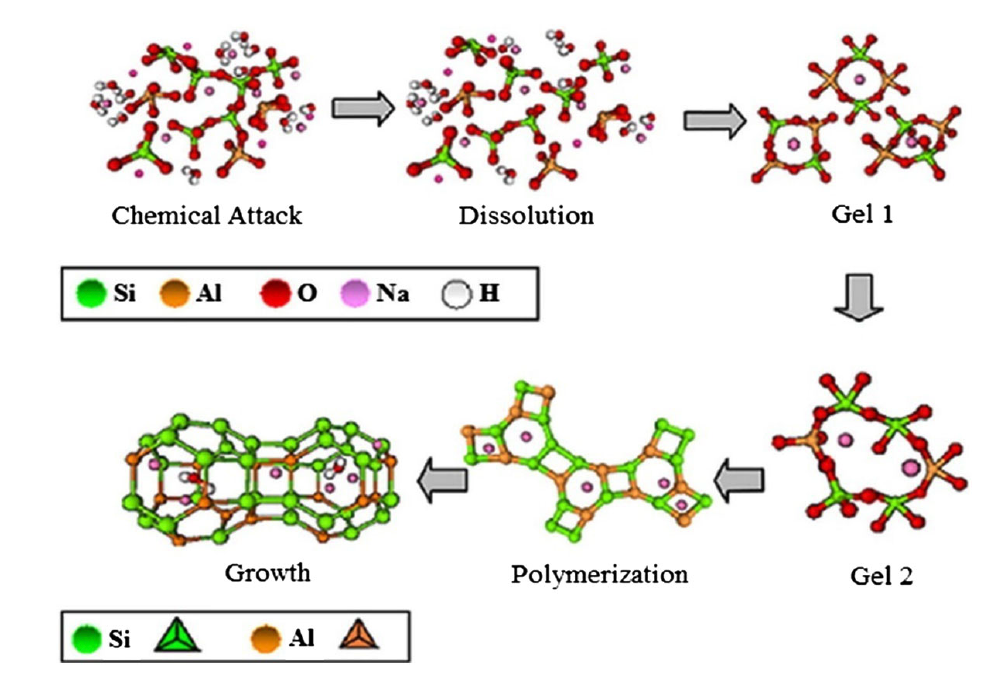
\includegraphics[width=0.75\textwidth]{Cap2/ativacao.png}
  \caption{Esquema do processo de ativação alcalina \cite{duxson2006geopolymer}.}
  \label{fig:ativacao}
\end{figure}

Os precursores podem ser divididos em duas categorias: os de alto teor de cálcio, como a escória de alto-forno e a cinza volante, e os de baixo teor de cálcio, como o metacaulim.
A Figura \ref{fig:diagrama_ternario} apresenta os precursores mais comuns e suas respectivas composições químicas.

\begin{figure}[ht]
  \centering
  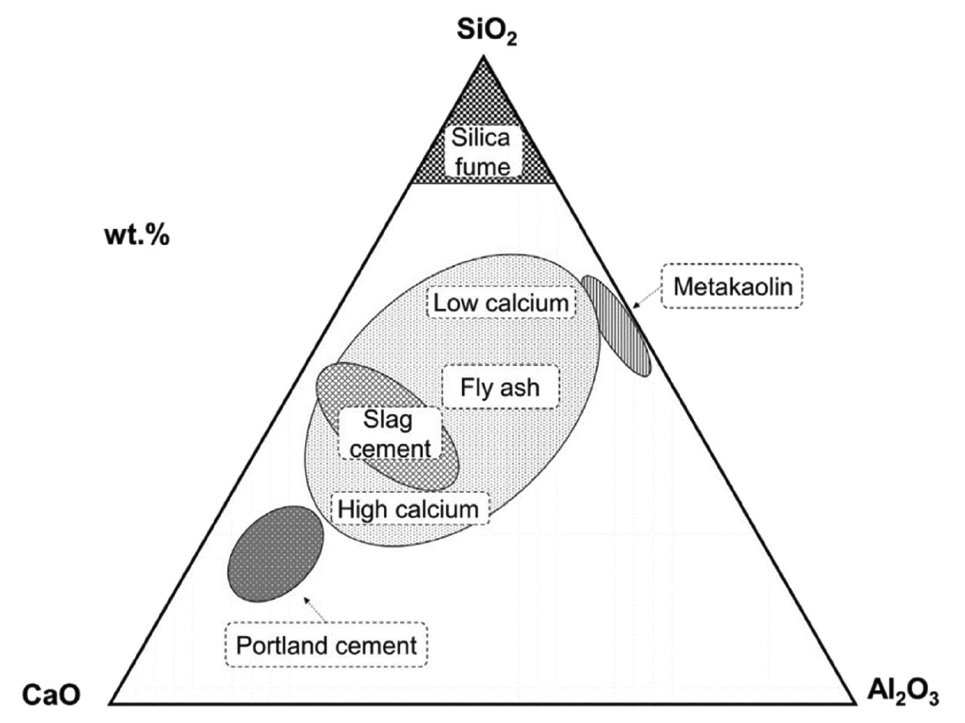
\includegraphics[width=0.625\textwidth]{Cap2/diagrama_ternario.png}
  \caption{Diagrama ternário dos precursores mais comuns \cite{giergiczny2019fly}.}
  \label{fig:diagrama_ternario}
\end{figure}

O primeiro grupo tem como principal produto da reação de ativação o silicato de alumínio e cálcio hidratado (C-A-S-H), enquanto o segundo grupo forma predominantemente o gel de silicato de alumínio hidratado (N-A-S-H).

Quando os níveis de cálcio presentes nesses precursores são elevados, o produto final é um gel de cura rápida e alta resistência inicial. No entanto, esses sistemas são mais suscetíveis a retrações, fissuras e corrosão por ataque de cloretos.
Já os sistemas de baixo cálcio formam uma rede amorfa de tetraedros, que apresenta baixa permeabilidade e retração, melhor resistência ao fogo e estrutura menos porosa.
A proporção de $SiO_2/Al_2O_3$ é responsável pelo grau de polimerização do gel formado; portanto, caso a relação ideal não seja atingida, a resistência mecânica e a durabilidade do AAM podem ser comprometidas.
Por fim, o gel N-A-S-H necessita de um maior tempo de cura e temperatura entre $80-100\ ^\circ C$ para atingir a resistência mecânica apropriada \cite{Nodehi2021}.

A Tabela \ref{tab:principais_precursores} apresenta as principais características dos precursores mais comuns.

\begin{landscape}
\begin{table}[p]
  \centering
  \caption{Características de materiais residuais comuns ou inovadores que podem ser adicionados ao concreto para produzir aglomerantes mais sustentáveis \cite{Nodehi2021}.}
  \vspace{0.5cm}
  {\small % Reduzir o tamanho da fonte para a tabela
  \renewcommand{\arraystretch}{1.2} % Aumentar o espaçamento entre linhas
  \begin{tabular}{p{3.5cm} p{3cm} p{2cm} p{2cm} p{4cm} p{6cm}}
    \hline
    Nome do aditivo & Forma usual & Densidade média (kg/m\textsuperscript{3}) & Tamanho médio partícula (\textmu m) & Limitações & Benefícios \\
    \hline
    Cimento Portland (OPC) & Irregular e angular & 1440 & 0,15--20 & -- & -- \\
    Sílica ativa & Esférica & 2200 & 0,1--0,5 & Reduz trabalhabilidade e resistência inicial & Aumenta a compacidade, resistência mecânica e durabilidade \\
    Escória de alto-forno moída (GGBFS) & Angular com superfície rugosa & 1000--1300 & 1,25--250 & Baixa resistência inicial & Aumenta a durabilidade, melhora a ITZ e resistência a sulfatos \\
    Cinza volante (Fly ash) & Esférica & 540--860 & 0,5--300 & Baixa resistência inicial & Melhora a trabalhabilidade e a resistência a longo prazo \\
    Metacaulim & Porosa, lamelar e angular & 890 & 1--20 & Reduz a trabalhabilidade & Preenche a microestrutura e melhora a ITZ \\
    Cinza de casca de arroz & Irregular com alta porosidade & 504--700 & 5--10 & Variação nas propriedades e baixa reatividade & Alto teor de sílica; melhora a compacidade e resistência \\
    Pó de vidro & Irregular & 2500 & 0,8--50 & Alta contaminação & Melhora a durabilidade e reação pozolânica \\
    Lama vermelha (red mud) & Irregular e em forma de agulha & 2700--3400 & 100 até mais de 200 & Alta contaminação & Alto teor de alumina, pode melhorar a hidratação \\
    Resíduos cerâmicos & Angular & ~1700 & Abaixo de 100 & -- & Melhora a compacidade e o desempenho \\
    Escória de incineração de resíduos sólidos urbanos (MSWI) & Irregular & 660--1690 & -- & -- & Melhora a microestrutura e reduz a porosidade \\
    Cinza de lodo de papel & Irregular & Abaixo de 100 & -- & -- & Ajusta favoravelmente a razão S/A \\
    \hline
  \end{tabular}
  }
\label{tab:principais_precursores}
\end{table}
\end{landscape}

% \subsubsection{Metacaulim}

% \subsubsection{Sílica ativa}

\subsection{Ativadores}

O ataque alcalino sobre a microestrutura dos precursores resulta na liberação de silicatos e aluminatos na solução.
A solubilidade da sílica e da alumina em função do pH é apresentada na Figura \ref{fig:solubilidade}.

\begin{figure}[ht]
  \centering
  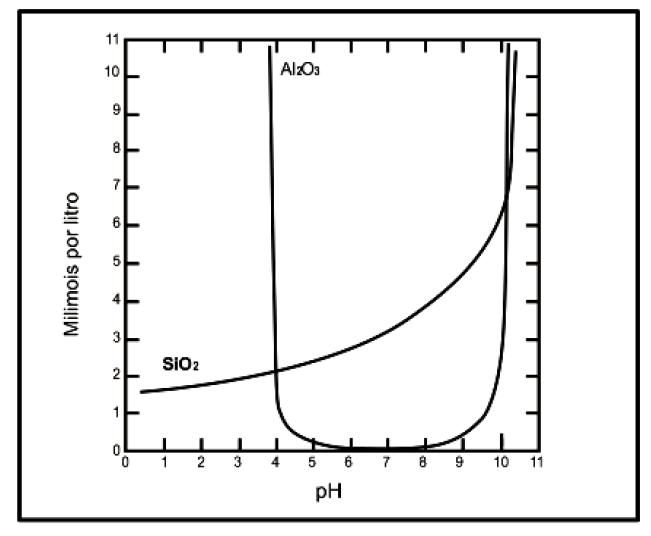
\includegraphics[width=0.625\textwidth]{Cap2/solubilidade.png}
  \caption{Solubilidade da sílica e da alumina em função do pH \cite{mason1952principles}.}
  \label{fig:solubilidade}
\end{figure}

Observa-se que a solubilidade da sílica é baixa em ambientes ácidos e elevada em meios básicos, enquanto a alumina é solúvel em ambos os extremos de pH.
Portanto, para que as reações de ativação ocorram, é necessário que o pH da solução seja elevado.

Os ativadores alcalinos podem ser encontrados em duas formas: líquida — produzindo os geopolímeros de duas partes — ou sólida — geopolímeros de uma parte.
Os principais ativadores alcalinos líquidos são: hidróxido de sódio ($NaOH$), silicato de sódio ($Na_2SiO_3$), hidróxido de potássio ($KOH$), carbonato de sódio ($Na_2CO_3$), carbonato de potássio ($K_2CO_3$) e óxido de potássio ($K_2O$).
Os primeiros estudos de AAM focaram em ativadores líquidos, uma vez que o produto final apresenta alta resistência à compressão, aderência e capacidade de suportar cargas de fadiga. Além disso, também demonstram elevada resistência a ciclos de congelamento e descongelamento e a altas temperaturas \cite{heath2014gwp}.

Apesar das vantagens dos sistemas de duas partes, as soluções básicas são corrosivas e irritam a pele humana, tornando seu transporte e manuseio perigosos para os trabalhadores \cite{awoyera2019critical}.
Outro ponto que merece atenção é que a produção de silicato de sódio ocorre entre $1200-1400\ ^\circ C$ e emite aproximadamente 1,514 kg de $CO_2$ por kg de silicato produzido, além de contribuir significativamente para a poluição do ar por meio de poeira e óxidos de nitrogênio e enxofre \cite{rajan2020sustainable}.

Dessa forma, os sistemas de uma parte surgem como uma alternativa mais segura, uma vez que os ativadores sólidos são menos perigosos e mais fáceis de manusear. Mesmo que os geopolímeros de uma parte apresentem menor resistência mecânica e necessitem de cura térmica para atingir o desempenho adequado \cite{provis2018alkali}, seu uso é mais escalável.

\section{Impactos Ambientais}

A principal vantagem ambiental atribuída aos AAMs reside na redução considerável de emissões de $CO_2$ em comparação com o cimento Portland tradicional.
Estima-se que os impactos ambientais dos ativadores sólidos e líquidos sejam de 24\% e 60\% do impacto causado pelo OPC, respectivamente \cite{luukkonen2017review}.
Além disso, a produção de AAMs frequentemente utiliza resíduos industriais como matérias-primas, como escória de alto forno, cinza de lodo de esgoto, de casca de arroz, de palha de cana-de-açúcar, entre outros \cite{moraes2024scsa}.
Portanto, além da valorização de resíduos industriais, a produção de AAMs reduz a demanda por recursos naturais de jazidas minerais e oferece uma destinação ambiental adequada, seguindo as propostas da Política Nacional de Resíduos Sólidos \cite{PNRS2016}.

\section{Propriedades Mecânicas}

